\section{Dynamisches Modell}

Das dynamische Modell beschreibt die Interaktionen zwischen den Entit�ten des statischen Modells.

\subsection{Neuer Spieler tritt bei}
Wenn eine neuer Spieler dem Spiel beitritt, muss er sich zun�chst beim Server melden. Dieser erstellt ein neues
Spieler-Objekt und informiert die bereits vorhandenen Client-Instanzen �ber den Beitritt und die Daten des neuen
Spielers.

\begin{figure}[htbp]
\centering
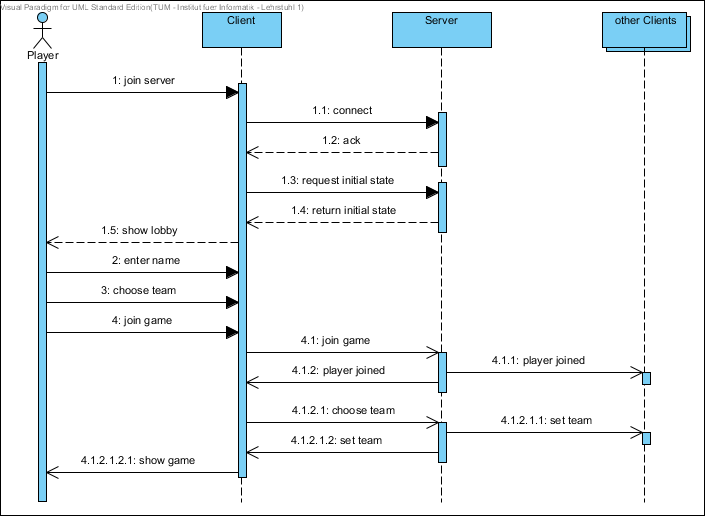
\includegraphics[width=1.0\textwidth]{images/sequence_player_joins}
\caption[Sequenzdiagramm "`Beitritt eines Spielers"']{Sequenzdiagramm "`Beitritt eines Spielers"'}
\label{sequence_player_joins}
\end{figure}


\subsection{Status�berg�nge im System}
Der Client, also die Spiel-Instanz des Spielers, durchl�uft verschiedene Zust�nde. Um alle n�tigen Zust�nde abzubilden
wurden zwei Statusvariablen implementiert: ClientState und GameState. Clientstate stellt den Zustand der Anwendung dar.
M�gliche Werte sind loading, lobby, menu und game. GameState bildet die m�glichen Zust�nde des Spiels ab: down, running,
spectate, roundover. Abbildung \ref{figure:state_machine} zeigt den Zusammenhang der Zust�nde als
Zustands-�bergangs-Diagramm.

\begin{figure}[htbp]
\centering
\includegraphics[width=1.0\textwidth]{images/state_machine}
\caption[Zustands-�bergangs-Diagramm]{Zustands-�bergangs-Diagramm}
\label{figure:state_machine}
\end{figure}